\documentclass{article}

\usepackage[english]{babel}
\usepackage[margin=3cm]{geometry}
\usepackage{graphicx}
\usepackage{float}
\usepackage{caption}
\usepackage{hyperref}
\usepackage{amsmath}
\usepackage{wrapfig}
\usepackage[parfill]{parskip}
\usepackage{eso-pic}

\usepackage{tcolorbox}


% fonts
\usepackage[T1]{fontenc}
\usepackage{helvet}
\renewcommand{\familydefault}{\sfdefault}

\graphicspath{{img/}}

% theorem environment
\usepackage{amssymb}

\newtheorem{theorem}{Definition}[section]

\usepackage{enumitem}

\newenvironment{thmenum}
 {\begin{enumerate}[label=\upshape\bfseries(\roman*)]}
 {\end{enumerate}}


% code
\usepackage{minted}
\setminted{frame=single,framesep=3pt,linenos}
\usepackage{upquote}
\usepackage{color}

\definecolor{titlepagecolor}{RGB}{68,200,245}

\begin{document}

\begin{titlepage}
    \pagecolor{titlepagecolor}
    \newgeometry{left=3cm,right=1cm,bottom=1cm}
    \noindent
\begin{flushright}
\vspace*{5cm}
 \vspace{2cm}
\end{flushright}
    \color{white}
    \par
    \noindent
    \color{white}
    \makebox[0pt][l]{\rule{1.3\textwidth}{1pt}}
    \par\medskip
    {\noindent \Huge\textbf{\textsf{Chess with Deep Reinforcement Learning: User Manual}}}
    \par\medskip
    {\noindent\Large\textsf{Tuur Vanhoutte}}
    \par  
\vfill%
\end{titlepage}
\restoregeometry
\nopagecolor

\pagenumbering{gobble}
\tableofcontents
\newpage

\pagenumbering{arabic}

\AddToShipoutPicture{
    \ifnum\value{page}>0
    \AtPageLowerLeft{
    \raisebox{3\baselineskip}{\makebox[0.25\paperwidth]{
        \begin{minipage}{21cm}\centering
            
\includegraphics{img/background.png}
        \end{minipage}}}
    }
  \fi
}

\section{Introduction}

I made a chess engine that uses deep reinforcement learning to 
play moves. It is possible to host the AI model on a GPU-equipped server, or
host the model locally.

This software has multiple features:

\begin{itemize}
	\item Create a training set using a specific AI model, by playing chess games against itself.
	\item Deploy a whole cluster of servers and clients to create a training set in parallel.
	\item Train the network using a training set created by self-play.
	\item Evaluate two different AI models by playing a given number of games against each other.
	\item Play against an AI
\end{itemize}


\section{Creating a training set}

To create a training set, you first need to either create your own AI model, or use my pretrained model.

\subsection{Create your own AI model}

To create your own AI model, run the following command:

\begin{minted}{shell}
python rlmodelbuilder.py --model-folder <FOLDER> --model-name <NAME> 

# For a detailed description of the parameters, run:
python rlmodelbuilder.py --help
\end{minted}

If you want to change parameters like the number of hidden layers, 
the input and output shapes (if you want to use the AI for other games), or the amount of convolution filters, 
change values in the config.py file.

\subsection{Use my pretrained model}

You can find a link to my pretrained model in the README.md file in the repository.
Copy the model.h5 file to the `models/' folder.

\subsection{Create a training set using the chosen model}

There are two ways to create a training set:

\begin{itemize}
	\item Play full chessgames with one model playing white, and a copy of the model playing black.
	\item Solve chess puzzles using the AI model.
\end{itemize}

The first method can easily be deployed using the docker-compose file:

\begin{minted}{shell}
# in repository's code/ folder:
docker-compose up --build
\end{minted}

This will deploy one prediction server and 8 clients $\Rightarrow$ 8 parallel games will play. 
The data for the training set will be stored in ./memory.
The amount of clients can be changed in the docker-compose file. 
You can also use the two docker images in a cluster like Kubernetes, to
reliably deploy many more servers and clients in parallel.

To manually run self-play or to solve puzzles, you can run the selfplay.py file 
with specific arguments. For a detailed description of the arguments, run:

\begin{minted}{shell}
python3 selfplay.py --help
\end{minted}

\subsubsection{Manual (non-dockerized) self-play with full games}

\begin{minted}{shell}
# if you want to send predictions to a server, start the server first:
python3 server.py
\end{minted}


\begin{minted}{shell}
# if you want to predict locally instead of on a server, add --local-predictions:
python3 selfplay.py --local-predictions
\end{minted}

The games will be saved in the './memory' folder.

\subsubsection{Solving puzzles (non-dockerized)}

You can download the puzzles file here: \url{https://database.lichess.org/#puzzles}.
This is a .csv file consisting of more than 2 million chess puzzles, 
with many different types (``mateIn1'', ``mateIn2'', ``endgame'', ``short'', etc\dots).

Training with these puzzles is faster than training with full games, and the AI can
more easily learn patterns like mating moves, or other patterns that are difficult to solve. 

\begin{minted}{shell}
python3 selfplay.py --type puzzles \
    --puzzle-file <PATH-TO-CSV-FILE> \
    --puzle-type <TYPE>
\end{minted}

Just like with self-play, you can add -{}-local-predictions if you want to predict locally instead of on a server.
If the puzzle ends in a checkmate within the move limit, the game will be saved to memory. That is why for now, only puzzles of type ``mateInX'' are supported.
The puzzle move limit can be changed in the config.py file.

\section{Training the AI using a created training set}

\begin{minted}{shell}
python3 train.py \
    --model <PATH-TO-MODEL> \
    --data-folder <PATH-TO-TRAINING-SET-FOLDER>

# For a full description of the parameters, run:
python3 train.py --help
\end{minted}

You can change parameters like batch size and learning rate in the config.py file. 

\section{Evaluating two models}

\begin{minted}{shell}
python3 evaluate.py evaluate.py <model_1> <model_2> <nr_games>

# For example, to run 100 matches between two models, run:
python3 evaluate.py models/model_1.h5 models/model_2.h5 100

# For a full description of the parameters, run:
python3 evaluate.py --help
\end{minted}

The white player in chess inherently has a slightly higher chance of winning,
because they can play the first move. Therefore, to evaluate two models, 
each model has to play as white and black an equal amount of games.

Therefore, running $n$ matches means the evaluation will consist of $2\cdot n$ games, because
each model will play both colors once per match.

The output of this command will be an overview of the results of the matches:

\begin{minted}{text}
Evaluated these models for 100 matches: 
    Model 1 = models/model_1.h5, Model 2 = models/model_2.h5 
The results: 
Model 1: X wins
Model 2: X wins
Draws: X
\end{minted}

\section{Playing against the AI}

To play against the AI, you can run the following command:

\begin{minted}{shell}
# [brackets] indicate optional arguments
python3 main.py [--player <white|black>] \
    [--local-predictions] \
    [--model <PATH-TO-MODEL>]
\end{minted}


\begin{itemize}
    \item If you don't specify a player, a random side will be chosen for you.
    \item If you add -{}-local-predictions, you also have to specify a model.
\end{itemize}

\begin{figure}[H]
    \centering
    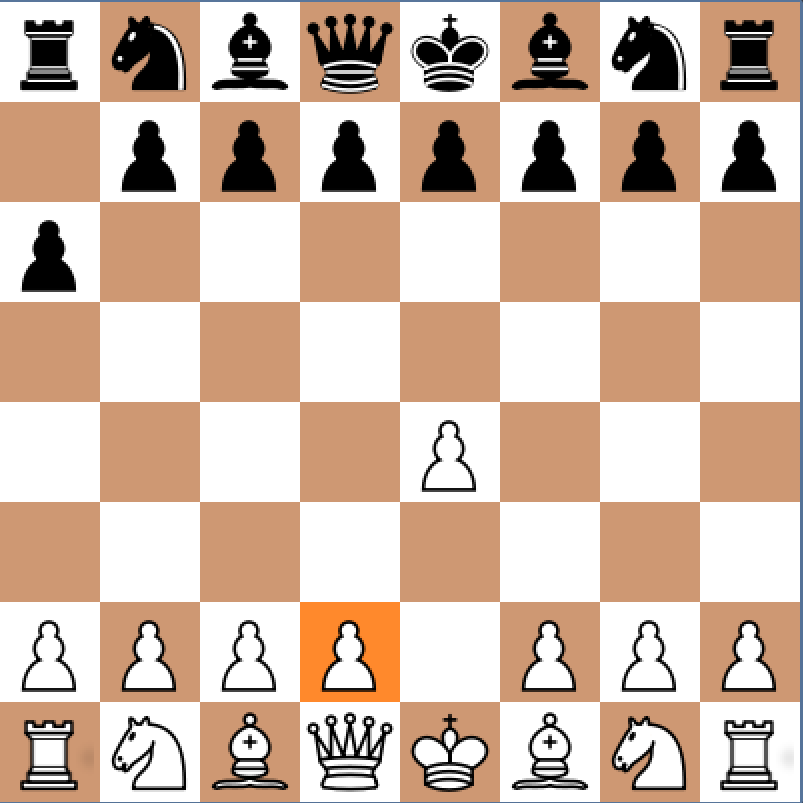
\includegraphics[width=0.5\textwidth]{img/chessboard-gui.png}
    \caption{The chessboard GUI}
\end{figure}

\begin{itemize}
    \item You can click on a piece to move it, then click a destination square
    \item When you click a piece, the square lights up to show it is selected 
\end{itemize}

\begin{figure}[H]
    \centering
    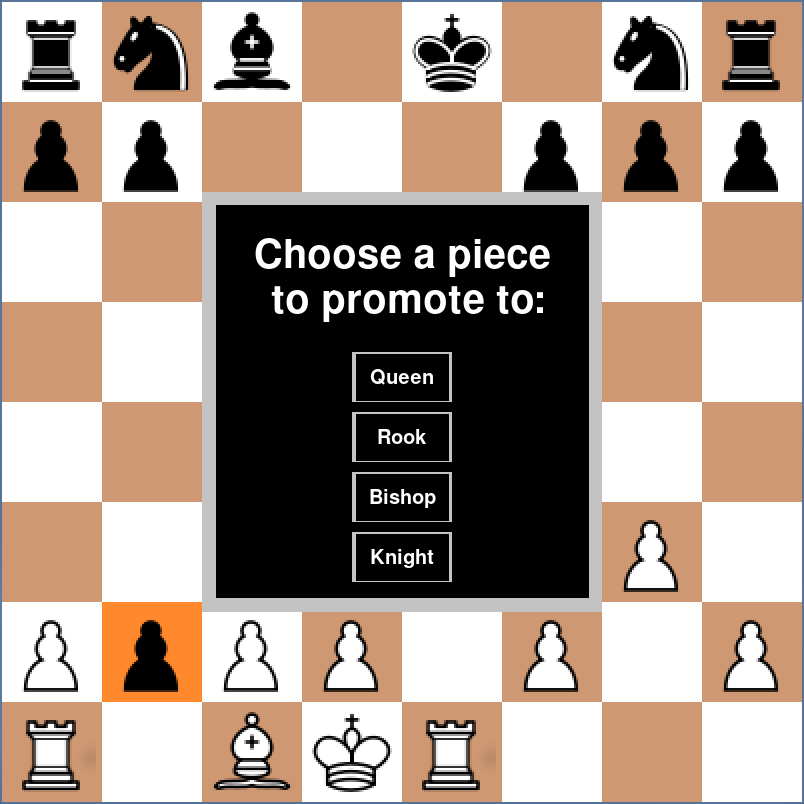
\includegraphics[width=0.5\textwidth]{img/chessboard-promotion.png}
    \caption{Promoting a pawn}
\end{figure}

\subsection{Changing the AI difficulty}

\begin{itemize}
    \item You can change the difficulty of the AI by changing the amount of MCTS simulations per move in the config.py file.
    \item This will also change the amount of time it takes for the AI to make a move.
\end{itemize}





\end{document}